\documentclass[pagesize,english,DIV=calc,footinclude=false
]{scrartcl}

\usepackage[utf8]{inputenc}
\usepackage[T1]{fontenc}
\usepackage[fleqn]{amsmath}
\usepackage[nohyperlinks]{acronym}
\usepackage{babel,lmodern,graphicx,mathptmx,xspace,wasysym,microtype,booktabs,tabularx,relsize,textcomp,longtable,lipsum,ifluatex,epstopdf}
\usepackage[olditem,oldenum]{paralist}
\usepackage[babel=true]{csquotes}
\usepackage[thinqspace]{SIunits}
\usepackage[normal,font=small]{caption}
\usepackage{subcaption}
\usepackage[multiple,flushmargin]{footmisc}
\usepackage{todonotes}
\usepackage{geometry}
\geometry{margin=1.2in}

\usepackage{url}
\urlstyle{same}

\usepackage{hyperref}
\hypersetup{
  pdftitle=Title,
  pdfkeywords={},
  pdfauthor=Author 1,
  plainpages=false,
  linktoc=all,
  colorlinks=true,
  anchorcolor=black,
  menucolor=black,
  linkcolor=black,
  citecolor=black,
  urlcolor=black,
  filecolor=black,
}

\graphicspath{{figures/}}
\DeclareGraphicsExtensions{.pdf,.jpeg,.png,.eps}         % Fix sort order in case the same file exists with multiple extensions
\frenchspacing

\ifluatex\else
% textcomp defines 00B1 wrong, so fix it here
\DeclareUnicodeCharacter{2192}{\ensuremath{\rightarrow}}
\DeclareUnicodeCharacter{2194}{\ensuremath{\leftrightarrow}}
\DeclareUnicodeCharacter{2212}{\ensuremath{-}}
\DeclareUnicodeCharacter{22EE}{\ensuremath{\vdots}}
\DeclareUnicodeCharacter{22EF}{\ensuremath{\cdots}}
\DeclareUnicodeCharacter{00B1}{\ensuremath{\pm}}
\DeclareUnicodeCharacter{00D7}{\ensuremath{\times}}
\DeclareUnicodeCharacter{221E}{\ensuremath{\infty}}
\DeclareUnicodeCharacter{2248}{\ensuremath{\approx}}
\DeclareUnicodeCharacter{2264}{\ensuremath{\leq}}
\DeclareUnicodeCharacter{2265}{\ensuremath{\geq}}
\DeclareUnicodeCharacter{03BC}{\micro}
\DeclareUnicodeCharacter{2206}{\ensuremath{\Delta}}
\fi

\newcommand{\m}[1]{\todo[noline,bordercolor=orange!20,backgroundcolor=orange!20]{#1}}

\newcommand{\eg}{e.\,g.\xspace}
\newcommand{\ie}{i.\,e.\xspace}

\addunit{\octave}{octave}
\addunit{\pbdrunit}{\%BDR}
\addunit{\plbdrunit}{\%LBDR}
\addunit{\currentunit}{cu}
\addunit{\pulsespersecondunit}{pps}

\newcommand{\pps}[1]{\unit{#1}{\pulsespersecondunit}}
\newcommand{\hz}[1]{\unit{#1}{\hertz}}
\newcommand{\khz}[1]{\unit{#1}{\kilo\hertz}}
\newcommand{\mhz}[1]{\unit{#1}{\mega\hertz}}
\newcommand{\db}[1]{\unit{#1}{\deci\bel}}
\newcommand{\us}[1]{\unit{#1}{\micro\second}}
\newcommand{\ms}[1]{\unit{#1}{\milli\second}}
\newcommand{\s}[1]{\unit{#1}{\second}}
\newcommand{\pc}[1]{\unit{#1}{\%}}
\newcommand{\pmil}[1]{\unit{#1}{\permil}}
\newcommand{\pcdb}[1]{\unit{#1}{\%\per\deci\bel}}
\newcommand{\de}[1]{\unit{#1}{\degree}}
\newcommand{\uv}[1]{\unit{#1}{\micro\volt}}
\newcommand{\nv}[1]{\unit{#1}{\nano\volt}}
\newcommand{\bdr}[1]{\unit{#1}{\pbdrunit}}
\newcommand{\lbdr}[1]{\unit{#1}{\plbdrunit}}
\newcommand{\cu}[1]{\unit{#1}{\currentunit}}
\newcommand{\nhl}[1]{\unit{#1}{\deci\bel{}\textnormal{nHL}}}
\newcommand{\hl}[1]{\unit{#1}{\deci\bel{}\textnormal{HL}}}
\newcommand{\spl}[1]{\unit{#1}{\deci\bel{}\textnormal{SPL}}}
\newcommand{\spla}[1]{\unit{#1}{\deci\bel{}\textnormal{SPL(A)}}}
\newcommand{\dbfs}[1]{\unit{#1}{\deci\bel{}\textnormal{FS}}}
\newcommand{\pespl}[1]{\unit{#1}{\deci\bel{}\textnormal{peSPL}}}
\newcommand{\pespla}[1]{\unit{#1}{\deci\bel{}\textnormal{peSPL(A)}}}
\newcommand{\sd}[1]{\ensuremath{\textnormal{SD}=#1}}
\newcommand{\se}[1]{\ensuremath{\textnormal{SE}=#1}}
\newcommand{\ir}[1]{\ensuremath{\textnormal{IR}=#1}}
\newcommand{\el}[2]{\ensuremath{\textnormal{#1}_{\textnormal{#2}}}}

% pandoc >=1.14
\providecommand{\tightlist}{\setlength{\itemsep}{0pt}\setlength{\parskip}{0pt}}


\usepackage[normalem]{ulem}
\pdfstringdefDisableCommands{\renewcommand{\sout}{}}


\setcounter{secnumdepth}{1}

\title{Selected Topics in Biomedical Signal Processing}
\author{Author 1 \and Author 2}
\date{Date}

\begin{document}

\maketitle

\section{Data-driven filter design for biomedical sensor arrays}

\subsection{Unsupervised artifact removal using CCA}

The raw EEG data is shown in Figure.\ref{fig:raw_eeg}. In Figure.\ref{fig:arti_zoom}, the eye-blink artifacts can be seen at $t=0s, 2.5s, 4.8s, 7.2s$. 

\begin{figure}[htbp]
  \centering
  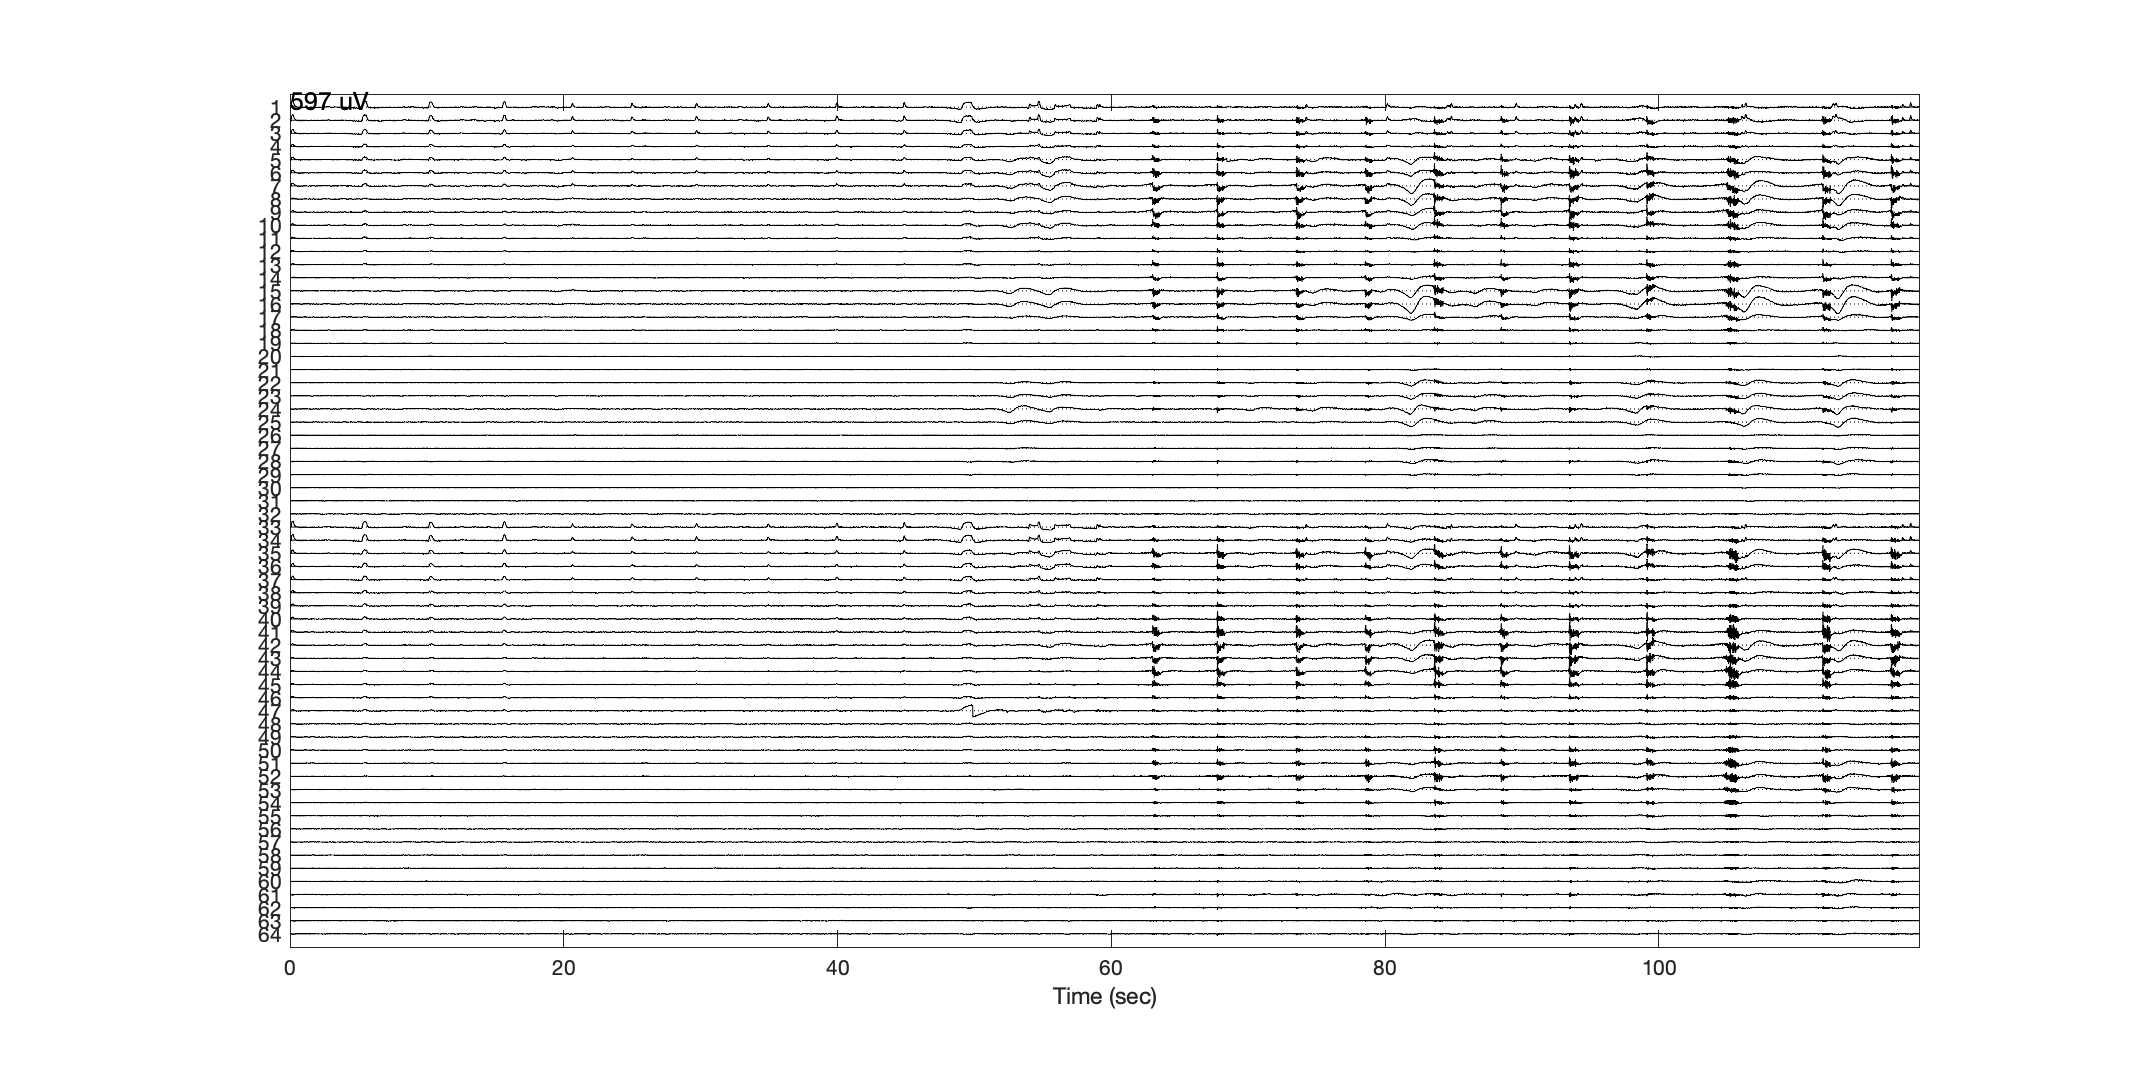
\includegraphics[width=\linewidth]{eeg_raw.eps}
  \caption{Raw EEG data}
  \label{fig:raw_eeg}
\end{figure}

The magnitude of the eye-blink artifacts differs from channel to channel. This is cause by the different locations of the electrodes.

\begin{figure}[htbp]
  \centering
  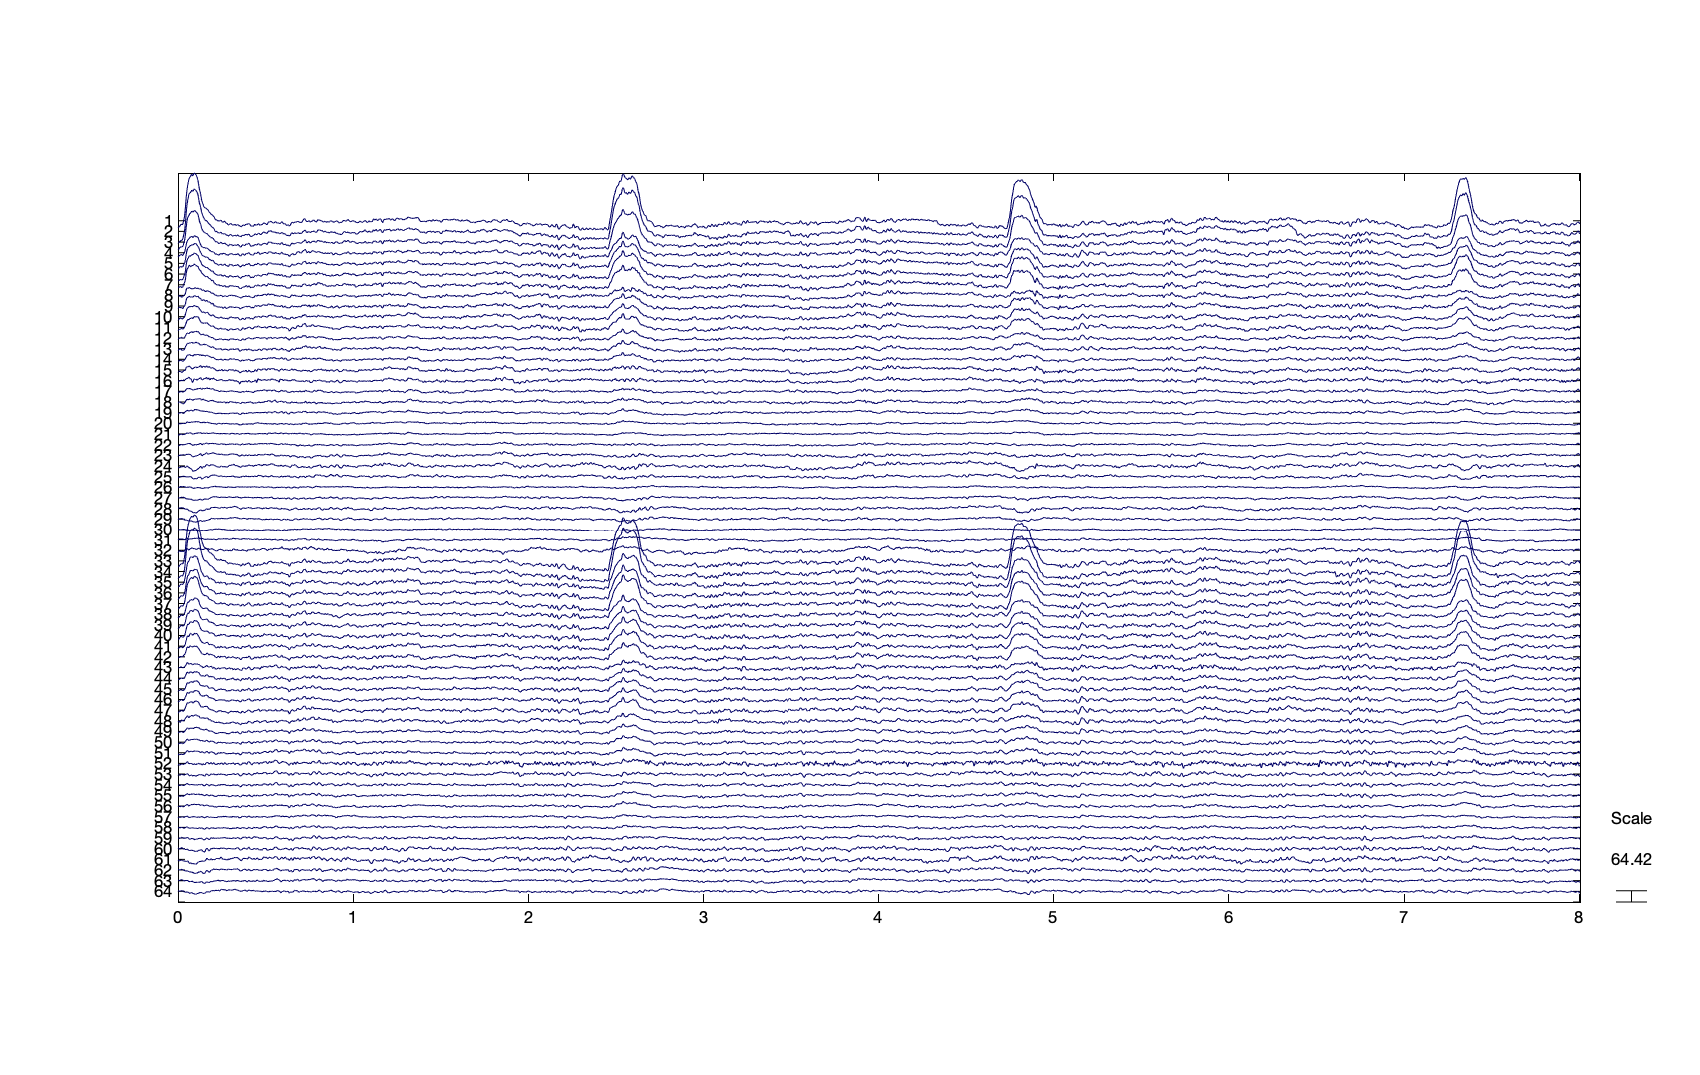
\includegraphics[width=\linewidth]{arti.eps}
  \caption{Eye-blink artifacts}
  \label{fig:arti_zoom}
\end{figure}


\begin{figure}[htbp]
  \centering
  \begin{subfigure}[b]{0.48\linewidth}
    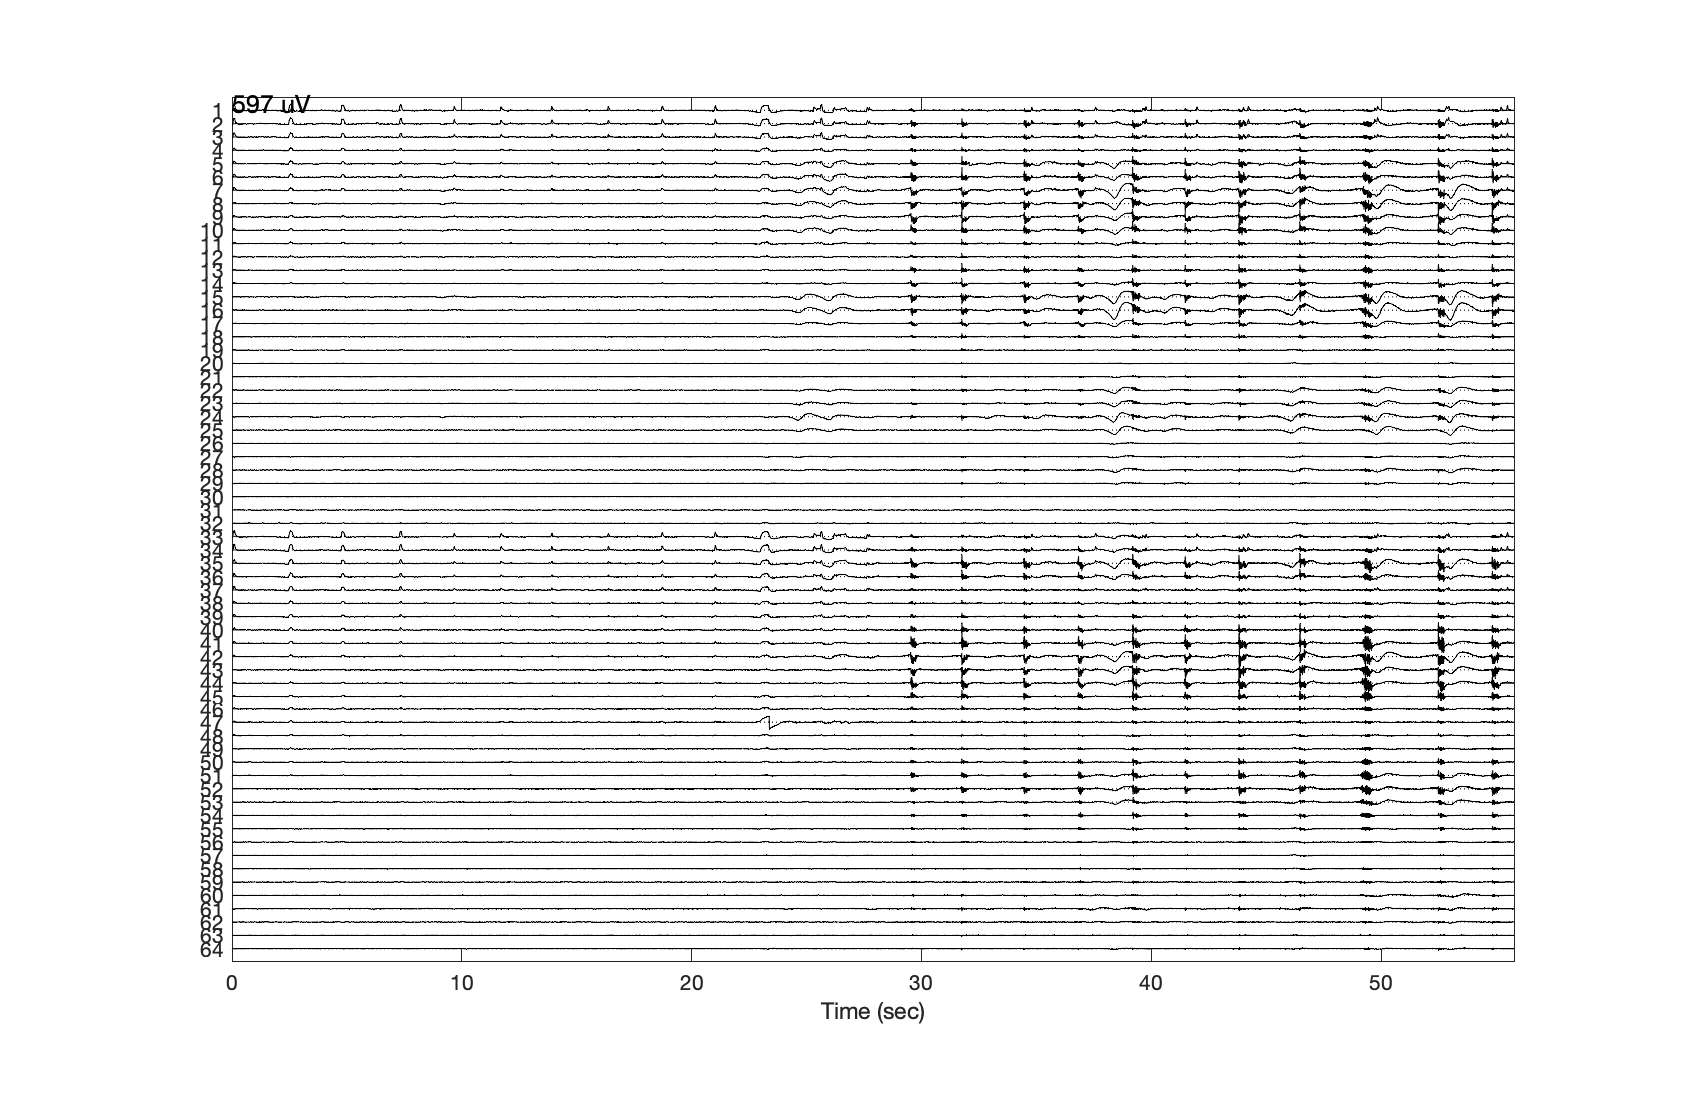
\includegraphics[width=\linewidth]{eeg_arti.eps}
    \caption{Raw EEG data}
  \end{subfigure}
  \begin{subfigure}[b]{0.48\linewidth}
    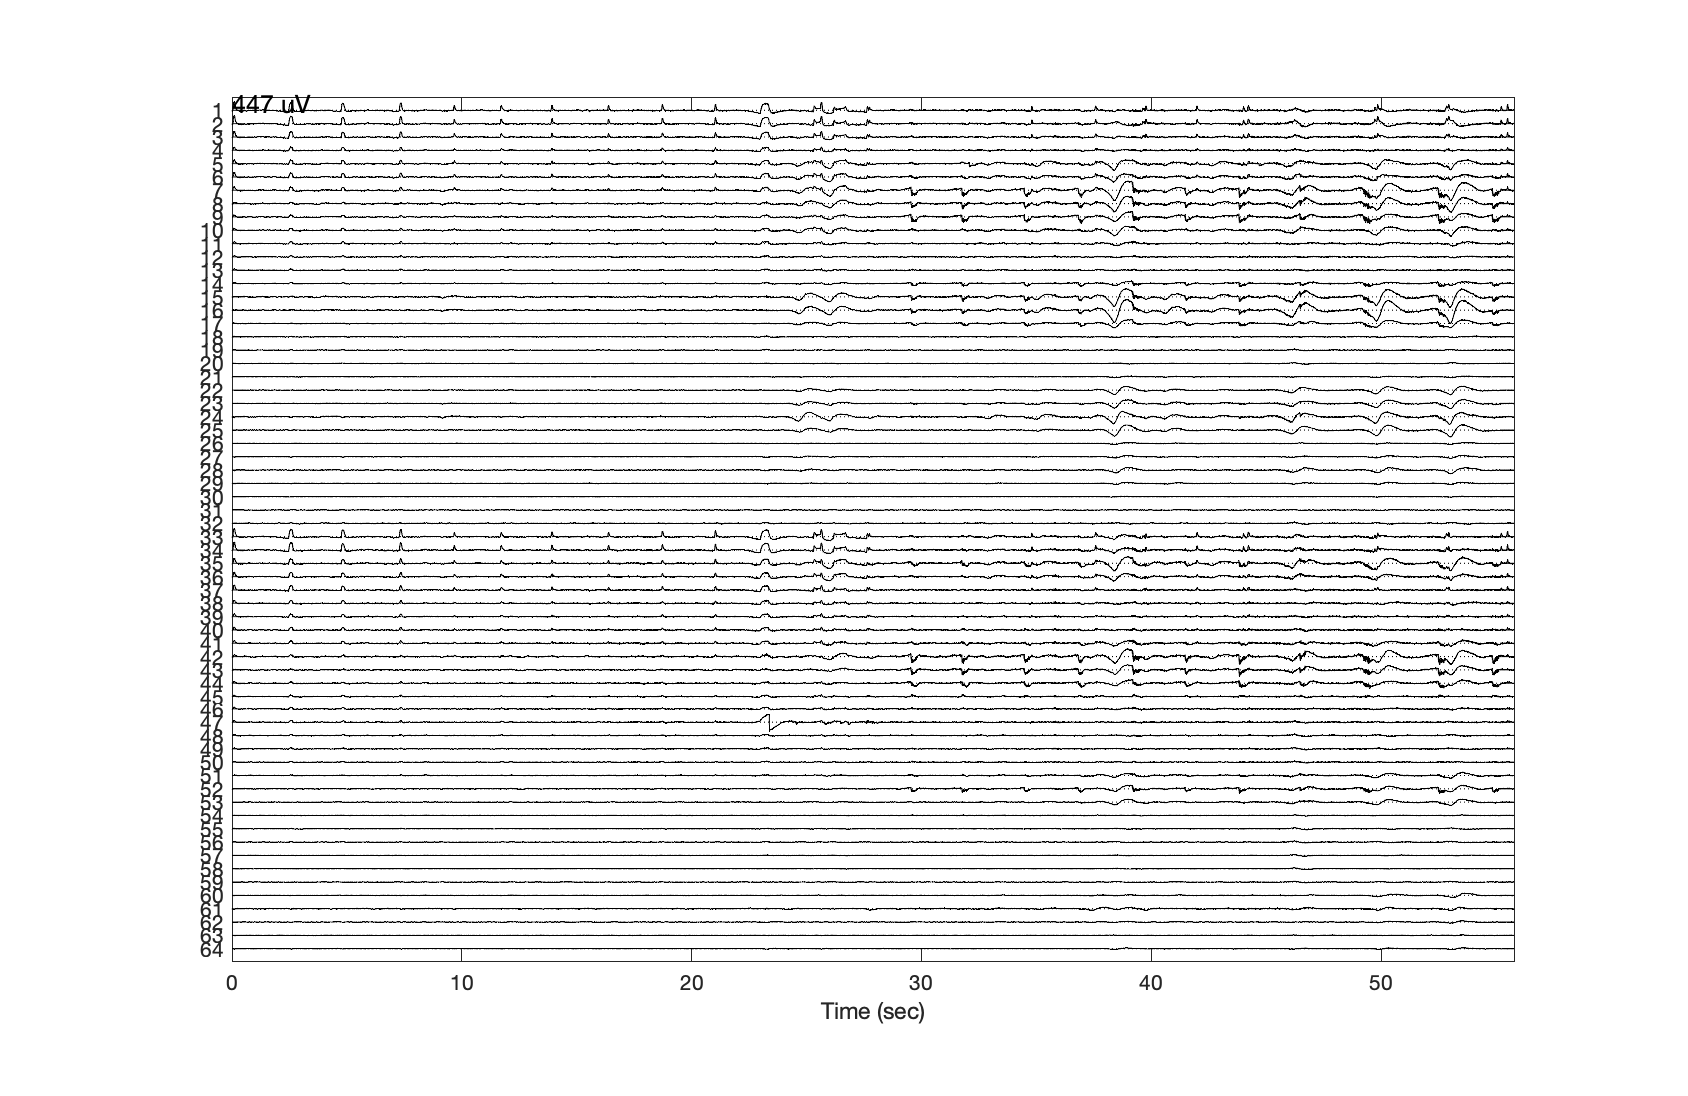
\includegraphics[width=\linewidth]{eeg_arti_rmv.eps}
    \caption{Muscle artifact removed}
  \end{subfigure}
  \caption{Artifact removel with CCA}
  \label{fig:arti_rmv}
\end{figure}

The reconstruction can be done by setting the sources with lower autocorrelation to 0.

\subsection{Supervised artifact removal using MWF}

\begin{figure}[htbp]
  \centering
  \begin{subfigure}[b]{0.48\linewidth}
    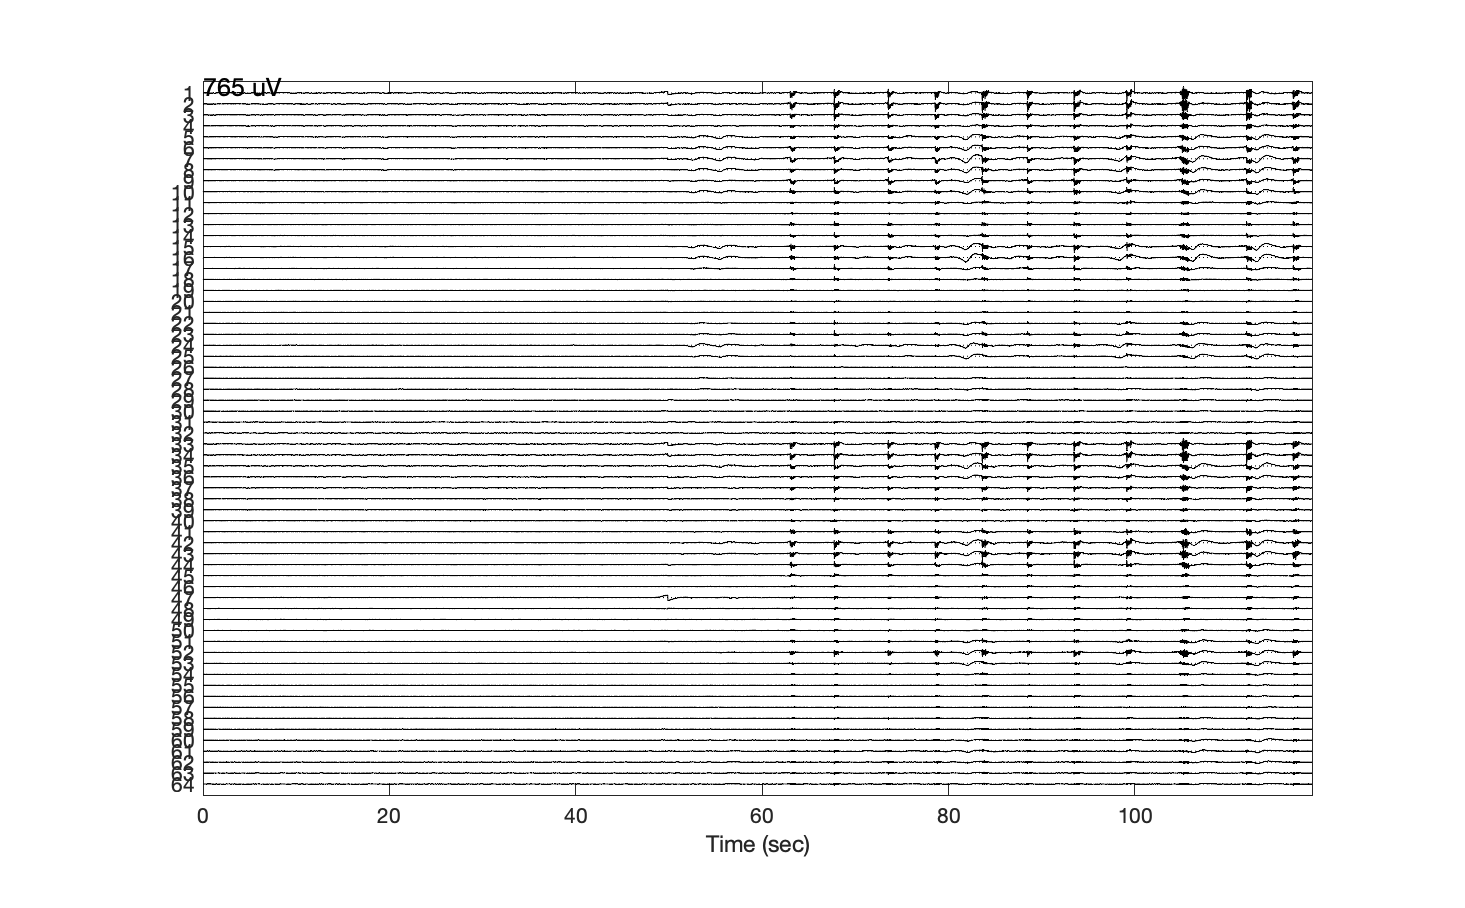
\includegraphics[width=\linewidth]{blink_arti_rmv.eps}
    \caption{Eye-blink artifact removal}
  \end{subfigure}
  \begin{subfigure}[b]{0.48\linewidth}
    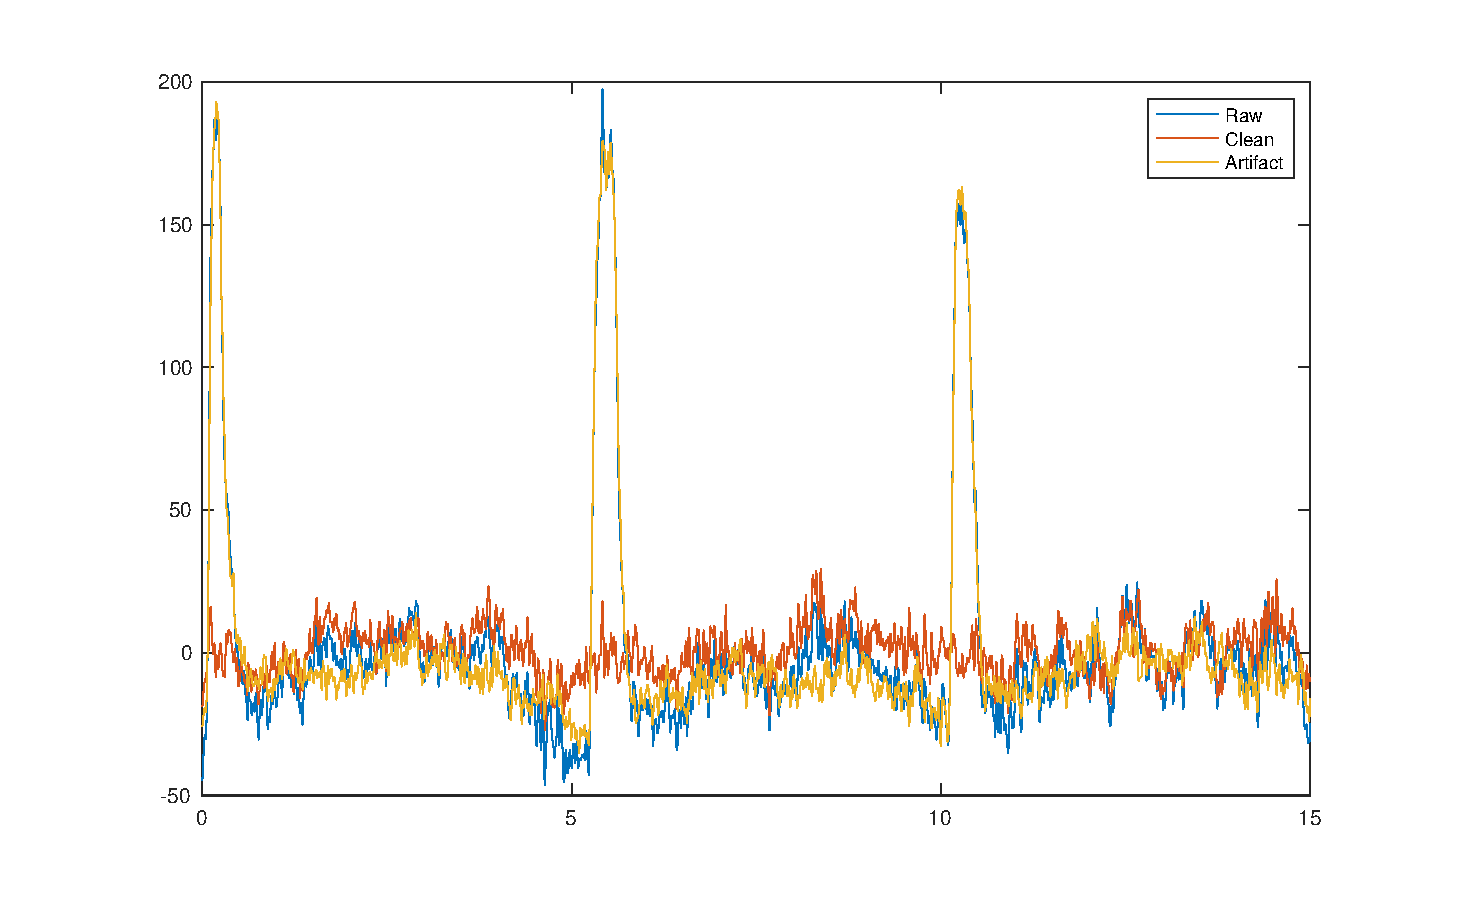
\includegraphics[width=\linewidth]{blink_arti_ch3.eps}
    \caption{Artifacts removal on Ch3, zoomed in}
  \end{subfigure}
  \caption{Eye-blink artifacts removal with MWF}
  \label{fig:blink}
\end{figure}

\begin{figure}[htbp]
  \centering
  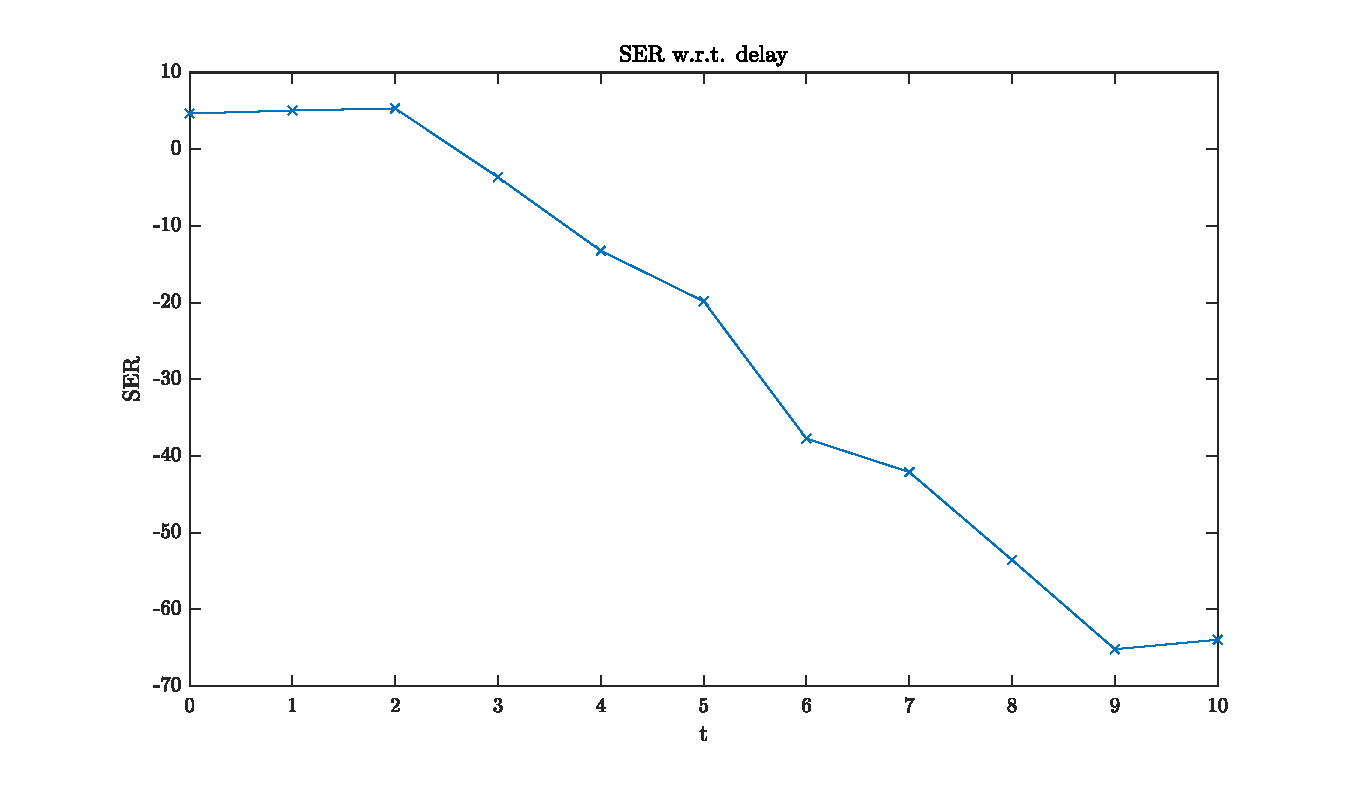
\includegraphics[width=0.7\linewidth]{mwf_delay_ser.eps}
  \caption{SER under different time delay}
  \label{fig:ser_delay}
\end{figure}



\section{Blind Signal Separation}


\end{document}
